\subsubsection{Vi phân tự động}
Vi phân tự động là một phương pháp tính toán cho phép xác định đạo hàm của các hàm số được biểu diễn thông qua một chuỗi hữu hạn các phép toán số học cơ bản và các hàm sơ cấp. Phương pháp này có vai trò quan trọng trong tính toán khoa học, tối ưu hóa và học sâu, đặc biệt trong việc tính đạo hàm của hàm mất mát đối với các tham số của mạng nơ-ron.

Ý tưởng cơ bản của vi phân tự động dựa trên thực tế rằng một phép tính số học dù phức tạp đến đâu cũng có thể được phân rã thành một số hữu hạn các phép toán cơ bản, chẳng hạn như phép cộng, phép trừ, phép nhân, phép chia, cùng với các hàm sơ cấp như hàm mũ, hàm logarit và các hàm lượng giác. Đạo hàm của từng phép toán và hàm sơ cấp này có thể được xác định trực tiếp. Bằng cách kết hợp các đạo hàm tương ứng theo quy tắc chuỗi, ta có thể xác định đạo hàm của toàn bộ hàm mà không cần khai triển toàn bộ biểu thức giải tích.

Để làm rõ cơ chế tính đạo hàm, xét một hàm hợp đơn giản:
$y =g_3\!\left(g_2\!\left(g_1(x)\right)\right).$

Đặt:
$$v_0 = x, \quad v_1 = g_1(v_0), \quad v_2 = g_2(v_1), \quad v_3 = g_3(v_2) = y.$$


Ở đây, $v_0$ là đại lượng đầu vào, $v_1, v_2$ là các đại lượng trung gian và $v_3=y$ là đại lượng đầu ra. Các đại lượng này tạo thành một chuỗi phụ thuộc:
\[
v_0 \longrightarrow v_1 \longrightarrow v_2 \longrightarrow v_3.
\]

Theo quy tắc chuỗi, đạo hàm của $y$ theo $x$ được xác định bởi:
\begin{equation}
\frac{\partial y}{\partial x} = \frac{\partial y}{\partial v_2} \frac{\partial v_2}{\partial v_1} \frac{\partial v_1}{\partial x}.
\end{equation}

Do $v_3 = y$, ta có thể viết:
\begin{equation}
\frac{\partial y}{\partial x} = \frac{\partial v_3}{\partial v_2} \frac{\partial v_2}{\partial v_1} \frac{\partial v_1}{\partial v_0}.
\end{equation}
Công thức trên cho thấy đạo hàm của hàm hợp có thể được tính bằng cách kết hợp các đạo hàm cục bộ từ những đại lượng trung gian trong quá trình tính toán. Vi phân tự động khai thác chính cấu trúc này để tính đạo hàm mà không cần xây dựng và khai triển toàn bộ biểu thức đạo hàm.

Có hai phương thức cơ bản để thực hiện vi phân tự động: \emph{chế độ thuận} và \emph{chế độ đảo}.
\begin{itemize}
    \item \textbf{Chế độ thuận:} Quá trình tính đạo hàm được thực hiện theo cùng chiều với quá trình tính giá trị, tức từ các đại lượng đầu vào đến đại lượng đầu ra.
    \[v_0 \longrightarrow v_1 \longrightarrow \cdots
    \longrightarrow v_n,\]
    trong đó $v_0=x$ là biến độc lập và $v_n=y$ là đại lượng đầu ra. Ta lần lượt tính đạo hàm của từng đại lượng trung gian theo $x$. Theo quy tắc chuỗi, ta có quan hệ truy hồi:
    $$\frac{\partial v_i}{\partial x}
    =\frac{\partial v_i}{\partial v_{i-1}}
    \frac{\partial v_{i-1}}{\partial x},\qquad i=1,\ldots,n.$$
    Sau khi thực hiện tuần tự các phép tính trên (với $v_n=y$), ta thu được:
    $$\frac{\partial y}{\partial x}
    =\frac{\partial v_n}{\partial x}.$$
    Để biểu diễn ngắn gọn đạo hàm được tích lũy tại mỗi đại lượng trung gian, đặt
    \[\dot{v}_i=\frac{\partial v_i}{\partial x},\qquad i=0,\ldots,n.\]
    Khi đó, quan hệ truy hồi được viết dưới dạng
    \[\dot{v}_i=\frac{\partial v_i}{\partial v_{i-1}}
    \dot{v}_{i-1},\qquad i=1,\ldots,n,\]
    với điều kiện khởi đầu
    \[\dot{v}_0=\frac{\partial v_0}{\partial x}=1.\]
    Như vậy, chế độ thuận lần lượt truyền đạo hàm từ biến độc lập $x$ qua các đại lượng trung gian $v_1,\ldots,v_{n-1}$ đến đại lượng đầu ra $y=v_n$. Đại lượng $\dot{v}_i$ biểu diễn sự biến thiên của $v_i$ theo biến độc lập $x$ và được tính dựa trên đạo hàm cục bộ
    $\partial v_i/\partial v_{i-1}$.
    
    \item \textbf{Chế độ đảo:} Quá trình tính đạo hàm ngược chiều với quá trình tính giá trị, tức từ đại lượng đầu ra về các đại lượng đầu vào.
    \[v_0 \longrightarrow v_1 \longrightarrow \cdots\longrightarrow v_n = y,\]
    
    trong đó $v_0=x$ là biến đầu vào và $v_n=y$ là đại lượng đầu ra. Ta bắt đầu từ đại lượng đầu ra $y$ và lần lượt tính đạo hàm của $y$ theo các đại lượng trung gian theo chiều ngược lại. Theo quy tắc chuỗi, ta có quan hệ truy hồi:
    \begin{equation}
    \frac{\partial y}{\partial v_i}
    =\frac{\partial y}{\partial v_{i+1}}
    \frac{\partial v_{i+1}}{\partial v_i},\qquad i=n-1,\ldots,0.
    \end{equation}
    
    Do $v_0=x$, tại bước cuối cùng ta thu được
    \begin{equation}
    \frac{\partial y}{\partial x}=\frac{\partial y}{\partial v_0}.
    \end{equation}
    
    Để biểu diễn ngắn gọn đạo hàm được tích lũy tại mỗi đại lượng trung gian, đặt
    \begin{equation}
    \overline{v}_i=\frac{\partial y}{\partial  v_i},\qquad i=0,\ldots,n.
    \end{equation}
    Khi đó, quan hệ truy hồi của quá trình tích lũy ngược được viết dưới dạng
    \begin{equation}
    \overline{v}_i=\overline{v}_{i+1}\frac{\partial v_{i+1}}{\partial v_i},\qquad i=n-1,\ldots,0,
    \end{equation}
    với điều kiện khởi đầu
    \begin{equation}
    \overline{v}_n=\frac{\partial y}{\partial v_n}=1.
    \end{equation}
\end{itemize}
Như vậy, chế độ ngược bắt đầu từ đại lượng đầu ra và lần lượt truyền đạo hàm về các đại lượng trung gian rồi đến các biến đầu vào. Trong đồ thị tính toán tổng quát, giá trị đạo hàm tích lũy tại một biến trung gian được xác định bằng tổng các đóng góp truyền ngược từ các nút phụ thuộc trực tiếp vào biến đó. Do đó, các đạo hàm theo nhiều biến đầu vào có thể được tính thông qua cùng một quá trình truyền ngược trên đồ thị tính toán.

\paragraph{So sánh hai chế độ tích lũy đạo hàm}

Xét ánh xạ tổng quát:
\begin{equation}
f: \mathbb{R}^n \rightarrow \mathbb{R}^m,
\end{equation}
trong đó $n$ và $m$ lần lượt là số chiều của không gian đầu vào và không gian đầu ra. Ký hiệu:
\begin{equation}
\mathbf{x} = (x_1, \dots, x_n)^{\top} \in \mathbb{R}^n, \qquad \mathbf{y} = f(\mathbf{x}) = (y_1, \dots, y_m)^{\top} \in \mathbb{R}^m.
\end{equation}
Ma trận đạo hàm của $f$ tại $\mathbf{x}$ được gọi là ma trận Jacobi, ký hiệu:
\begin{equation}
\mathbf{J}_f(\mathbf{x}) = \left[ \frac{\partial y_i}{\partial x_j} \right]_{\substack{i=1,\dots,m \\ j=1,\dots,n}} \in \mathbb{R}^{m \times n}.
\end{equation}

\begin{itemize}
    \item \textbf{Chế độ thuận:} Khi $n \ll m$, chế độ thuận phù hợp hơn vì mỗi lần tích lũy xuôi có thể cố định một biến đầu vào và tính đạo hàm của toàn bộ các đại lượng đầu ra theo biến đó. Cụ thể, với biến đầu vào $x_j$, quá trình tích lũy xuôi cho phép xác định đồng thời:
    \begin{equation}
    \frac{\partial y_1}{\partial x_j}, \frac{\partial y_2}{\partial x_j}, \dots, \frac{\partial y_m}{\partial x_j}.
    \end{equation}
    Các đạo hàm này tạo thành cột thứ $j$ của ma trận Jacobi:
    \begin{equation}
    \mathbf{J}_f(\mathbf{x})_{:,j} = 
    \begin{bmatrix}
    \dfrac{\partial y_1}{\partial x_j} \\
    \vdots \\
    \dfrac{\partial y_m}{\partial x_j}
    \end{bmatrix}.
    \end{equation}
    Do đó, để xác định toàn bộ ma trận Jacobi bằng chế độ thuận, cần thực hiện quá trình tích lũy xuôi tương ứng với từng biến đầu vào. Số lần tích lũy (số bước duyệt qua đồ thị) cần thiết là $n$.

    \item \textbf{Chế độ đảo:} Khi $n \gg m$, chế độ đảo phù hợp hơn vì mỗi lần tích lũy ngược có thể cố định một đại lượng đầu ra và tính đạo hàm của đại lượng đó theo toàn bộ các biến đầu vào. Cụ thể, với đầu ra $y_i$, quá trình tích lũy ngược cho phép xác định đồng thời:
    \begin{equation}
    \frac{\partial y_i}{\partial x_1}, \frac{\partial y_i}{\partial x_2}, \dots, \frac{\partial y_i}{\partial x_n}.
    \end{equation}
    Các đạo hàm này tạo thành hàng thứ $i$ của ma trận Jacobi:
    \begin{equation}
    \mathbf{J}_f(\mathbf{x})_{i,:} = 
    \begin{bmatrix}
    \dfrac{\partial y_i}{\partial x_1} & \cdots & \dfrac{\partial y_i}{\partial x_n}
    \end{bmatrix}.
    \end{equation}
    Do đó, để xác định toàn bộ ma trận Jacobi bằng chế độ đảo, cần thực hiện quá trình tích lũy ngược tương ứng với từng biến đầu ra. Số lần tích lũy cần thiết là $m$.
\end{itemize}

Từ đó, khi $n \ll m$, chế độ thuận tốn ít chi phí tính toán hơn; ngược lại, khi $n \gg m$, chế độ đảo lại tối ưu hơn. Sự khác biệt về số lần tích lũy là một cơ sở quan trọng để lựa chọn chế độ vi phân tự động phù hợp với số chiều của không gian đầu vào và đầu ra.


\paragraph{Mối liên hệ với lan truyền ngược trong mạng nơ-ron\\}
Đối với mạng nơ-ron có L lớp, các tham số của mô hình có thể được xem là các biến của một ánh xạ từ không gian tham số đến giá trị của hàm mất mát. Ký hiệu tập các tham số của mạng là
\begin{equation}
\boldsymbol{\Theta}
=
\left\{
\mathbf{W}^{[l]},\mathbf{b}^{[l]}
\right\}_{l=1}^{L},
\end{equation}
trong đó $\mathbf{W}^{[l]}$ và $\mathbf{b}^{[l]}$ lần lượt là ma trận trọng số và vectơ độ chệch của lớp thứ $l$, $l=1,...L$. 

Giả sử tổng số tham số của mạng là $N$. Khi sắp xếp toàn bộ các phần tử của các ma trận trọng số và các véc-tơ độ chệch theo một thứ tự xác định thành một véc-tơ duy nhất, ta thu được véc-tơ tham số:
\begin{equation}
\boldsymbol{\theta} =
\begin{bmatrix}
\theta_1 & \theta_2 & \cdots & \theta_N
\end{bmatrix}^{\mathsf T}
\in\mathbb{R}^{N}.
\end{equation}
Trong đó:
\begin{itemize}
    \item $\boldsymbol{\theta}$: Véc-tơ tham số của mạng, được tạo thành bằng cách sắp xếp toàn bộ các tham số của mạng thành một véc-tơ duy nhất.
    \item $\theta_i$: Tham số thứ $i$ của mạng ($i=1,\ldots,N$), tương ứng với một phần tử của ma trận trọng số hoặc véc-tơ độ chệch thuộc một lớp cụ thể.
    \item $N$: Tổng số tham số của mạng.
    \item $\mathsf{T}$: Phép chuyển vị ma trận/véc-tơ, qua đó chuyển véc-tơ hàng $\begin{bmatrix} \theta_1 & \theta_2 & \cdots & \theta_N \end{bmatrix}$ thành véc-tơ cột.
    \item $\mathbb{R}^{N}$: Không gian véc-tơ thực $N$ chiều; do đó, ký hiệu $\boldsymbol{\theta}\in\mathbb{R}^{N}$ cho biết véc-tơ tham số có $N$ thành phần thực.
\end{itemize}
Với hàm mất mát vô hướng $\mathcal{L}=\mathcal{L}(\boldsymbol{\theta}),$ có thể được xem như một ánh xạ:
\begin{equation}
\mathcal{L}:\mathbb{R}^{N}\rightarrow\mathbb{R}.
\end{equation}

Trong biểu diễn này, không gian đầu vào của ánh xạ có $N$ chiều, tương ứng với tổng số tham số của mạng, trong khi không gian đầu ra chỉ có một chiều do hàm mất mát nhận giá trị vô hướng. Vì số lượng tham số của mạng thường rất lớn, ta có: $N\gg 1.$


Do đó, bài toán tính đạo hàm của hàm mất mát trong lan truyền ngược thuộc trường hợp ánh xạ có số chiều đầu vào lớn hơn rất nhiều so với số chiều đầu ra. Trong trường hợp này, vi phân tự động chế độ đảo phù hợp hơn. Chỉ với \textbf{một lần} lan truyền ngược duy nhất, ta có thể tính được đạo hàm của hàm mất mát theo toàn bộ các tham số:
\begin{equation}
\frac{\partial \mathcal{L}}{\partial \theta_1}, \frac{\partial \mathcal{L}}{\partial \theta_2}, \dots, \frac{\partial \mathcal{L}}{\partial \theta_N}.
\end{equation}
Các đạo hàm vô hướng này sau đó được tái định dạng lại tương ứng với kích thước của ma trận trọng số và véc-tơ độ chệch tại từng lớp để thu được:
\begin{equation}
\frac{\partial \mathcal{L}}{\partial \mathbf{W}^{[l]}} \quad \text{và} \quad \frac{\partial \mathcal{L}}{\partial \mathbf{b}^{[l]}}, \qquad l = 1, \dots, L.
\end{equation}
Cơ chế này chính là cơ sở toán học của lan truyền ngược trong mạng nơ-ron.

Như vậy, vi phân tự động cung cấp một phương pháp tổng quát để tính đạo hàm dựa trên cấu trúc của đồ thị tính toán. Chế độ thuận truyền sự phụ thuộc của đạo hàm từ đầu vào đến đầu ra và đặc biệt phù hợp khi số chiều đầu vào nhỏ hơn đáng kể số chiều đầu ra. Ngược lại, chế độ đảo truyền sự phụ thuộc của đạo hàm từ đầu ra về đầu vào và là phương pháp phù hợp khi số chiều đầu vào lớn hơn đáng kể số chiều đầu ra. Lan truyền ngược trong học sâu chính là trường hợp áp dụng của chế độ đảo cho bài toán tính gradient của một hàm mất mát vô hướng theo tham số của mạng nơ-ron.
\paragraph{Minh họa tính toán cho vi phân tự động chế độ thuận và chế độ đảo\\}
Xét hàm vô hướng hai biến:
\begin{equation}
    y = f(x_1,x_2) = \ln(x_1) + x_1 x_2 - \sin(x_2).
    \label{eq:ad_example_function}
\end{equation}
Mục tiêu là tính véc-tơ đạo hàm:
\begin{equation}
    \nabla f(x_1,x_2) = 
    \begin{bmatrix}
        \dfrac{\partial y}{\partial x_1} \\[6pt]
        \dfrac{\partial y}{\partial x_2}
    \end{bmatrix}
\end{equation}
bằng hai phương thức của vi phân tự động: chế độ thuận và chế độ đảo.

\paragraph{Xây dựng đồ thị tính toán:\\}

Để áp dụng vi phân tự động, hàm \eqref{eq:ad_example_function} được phân rã thành một chuỗi các phép toán cơ bản. Đặt:
\begin{equation}
\begin{aligned}
    v_{-1} &= x_1, \\
    v_0 &= x_2, \\
    v_1 &= \ln(v_{-1}), \\
    v_2 &= v_{-1} v_0, \\
    v_3 &= \sin(v_0), \\
    v_4 &= v_1 + v_2, \\
    v_5 &= v_4 - v_3 = y.
\end{aligned}
\label{eq:ad_example_graph}
\end{equation}

Các đạo hàm cục bộ tương ứng là:
\begin{equation}
    \frac{\partial v_1}{\partial v_{-1}} = \frac{1}{v_{-1}},
\end{equation}
\begin{equation}
    \frac{\partial v_2}{\partial v_{-1}} = v_0, \qquad \frac{\partial v_2}{\partial v_0} = v_{-1},
\end{equation}
\begin{equation}
    \frac{\partial v_3}{\partial v_0} = \cos(v_0),
\end{equation}
và
\begin{equation}
    \frac{\partial v_4}{\partial v_1} = \frac{\partial v_4}{\partial v_2} = \frac{\partial v_5}{\partial v_4} = 1, \qquad \frac{\partial v_5}{\partial v_3} = -1.
\end{equation}
Đồ thị tính toán của hàm có cấu trúc:
\begin{equation}
    (x_1,x_2) \longrightarrow (v_1,v_2,v_3) \longrightarrow v_4 \longrightarrow y.
\end{equation}
Việc phân rã này cho phép tính các đạo hàm của hàm đầu ra theo các biến đầu vào bằng cách sử dụng các đạo hàm cục bộ tại từng nút của đồ thị tính toán.
\paragraph{Tính đạo hàm bằng chế độ thuận:\\}
Trong chế độ thuận, đạo hàm được truyền từ các biến đầu vào đến biến đầu ra. Với một biến độc lập $x_j$, đặt giá trị tiếp tuyến tại đỉnh $v_i$ là:
\begin{equation}
    \dot{v}_i = \frac{\partial v_i}{\partial x_j}.
\end{equation}
Các giá trị này được tính tuần tự theo chiều thuận của đồ thị.
\begin{itemize}
    \item \textit{Đạo hàm theo $x_1$:}
    Chọn $x_1$ làm biến độc lập. Khi đó:
    \begin{equation}
        \dot{v}_{-1} = \frac{\partial v_{-1}}{\partial x_1} = 1, \qquad \dot{v}_0 = \frac{\partial v_0}{\partial x_1} = 0.
    \end{equation}
    Tại đỉnh $v_1 = \ln(v_{-1})$:
    \begin{equation}
        \dot{v}_1 = \frac{\partial v_1}{\partial v_{-1}}\dot{v}_{-1} = \frac{1}{v_{-1}} = \frac{1}{x_1}.
    \end{equation}
    Tại đỉnh $v_2 = v_{-1} v_0$, áp dụng quy tắc đạo hàm của tích:
    \begin{equation}
    \begin{aligned}
        \dot{v}_2 &= \frac{\partial v_2}{\partial v_{-1}}\dot{v}_{-1} + \frac{\partial v_2}{\partial v_0}\dot{v}_0 \\
        &= v_0(1) + v_{-1}(0) = x_2.
    \end{aligned}
    \end{equation}
    Tại đỉnh $v_3 = \sin(v_0)$:
    \begin{equation}
        \dot{v}_3 = \frac{\partial v_3}{\partial v_0}\dot{v}_0 = \cos(v_0)(0) = 0.
    \end{equation} 
    Tiếp theo:
    \begin{equation}
        \dot{v}_4 = \dot{v}_1 + \dot{v}_2 = \frac{1}{x_1} + x_2.
    \end{equation}
    Cuối cùng, vì $v_5 = v_4 - v_3$:
    \begin{equation}
        \dot{v}_5 = \dot{v}_4 - \dot{v}_3 = \frac{1}{x_1} + x_2.
    \end{equation}
    Do $v_5 = y$, suy ra:
    \begin{equation}
        \frac{\partial y}{\partial x_1} = \frac{1}{x_1} + x_2.
        \label{eq:forward_dx1}
    \end{equation}

    \item \textit{Đạo hàm theo $x_2$:}
    Tiếp tục thực hiện một lượt tích lũy thuận với $x_2$ làm biến độc lập. Khi đó:
    \begin{equation}
        \dot{v}_{-1} = \frac{\partial v_{-1}}{\partial x_2} = 0, \qquad \dot{v}_0 = \frac{\partial v_0}{\partial x_2} = 1.
    \end{equation}
    Tại đỉnh $v_1 = \ln(v_{-1})$:
    \begin{equation}
        \dot{v}_1 = \frac{1}{v_{-1}}\dot{v}_{-1} = 0.
    \end{equation}
    Tại đỉnh $v_2 = v_{-1} v_0$:
    \begin{equation}
    \begin{aligned}
        \dot{v}_2 &= v_0\dot{v}_{-1} + v_{-1}\dot{v}_0 \\
        &= x_2(0) + x_1(1) = x_1.
    \end{aligned}
    \end{equation}
    Tại đỉnh $v_3 = \sin(v_0)$:
    \begin{equation}
        \dot{v}_3 = \cos(v_0)\dot{v}_0 = \cos(x_2).
    \end{equation}
    Tại đỉnh $v_4$:
    \begin{equation}
        \dot{v}_4 = \dot{v}_1 + \dot{v}_2 = x_1,
    \end{equation}
    và $v_5$
    \begin{equation}
        \dot{v}_5 = \dot{v}_4 - \dot{v}_3 = x_1 - \cos(x_2).
    \end{equation}
    Suy ra:
    \begin{equation}
        \frac{\partial y}{\partial x_2} = x_1 - \cos(x_2).
        \label{eq:forward_dx2}
    \end{equation}
    Từ \eqref{eq:forward_dx1} và \eqref{eq:forward_dx2}, véc-tơ đạo hàm thu được bằng chế độ thuận là:
    \begin{equation}
        \nabla f(x_1,x_2) = 
        \begin{bmatrix}
            \dfrac{1}{x_1} + x_2 \\[6pt]
            x_1 - \cos(x_2)
        \end{bmatrix}.
        \label{eq:forward_gradient}
    \end{equation}
    Có thể nhận thấy rằng để thu được toàn bộ véc-tơ đạo hàm của hàm $f:\mathbb{R}^2 \rightarrow \mathbb{R}$ bằng chế độ thuận, cần thực hiện hai lượt tích lũy, tương ứng với hai hướng độc lập $x_1$ và $x_2$.
\end{itemize}
Chi tiết quá trình tính toán theo chiều thuận và tích lũy giá trị các biến trung gian tại điểm $(x_1,x_2) = (2,5)$, với giá trị khởi tạo là $\dot{x}_1 = \dot{v}_{-1} = 1$ và $\dot{x}_2 = \dot{v}_0 = 0$.
\begin{table}[H]
\centering
\renewcommand{\arraystretch}{1.35}
\begin{tabular*}{\textwidth}{@{\extracolsep{\fill}} l l | l l @{}}
\hline
\multicolumn{2}{l|}{Chuỗi giá trị các biến tính toán} & \multicolumn{2}{l}{Chuỗi giá trị các biến trung gian} \\
\hline
$v_{-1} = x_1$        & $= 2$             & $\dot{v}_{-1} = \dot{x}_1$                             & $= 1$ \\
$v_0 = x_2$           & $= 5$             & $\dot{v}_0 = \dot{x}_2$                                & $= 0$ \\
$v_1 = \ln(v_{-1})$   & $\approx 0.693$   & $\dot{v}_1 = \dot{v}_{-1} / v_{-1}$                    & $= 1 / 2 = 0.5$ \\
$v_2 = v_{-1} \times v_0$& $= 2 \times 5 = 10$& $\dot{v}_2 = \dot{v}_{-1} \times v_0 + v_{-1} \times \dot{v}_0$ & $= 1 \times 5 + 2 \times 0 = 5$ \\
$v_3 = \sin(v_0)$     & $\approx -0.959$  & $\dot{v}_3 = \dot{v}_0 \cos(v_0)$                      & $= 0 \times \cos(5) = 0$ \\
$v_4 = v_1 + v_2$     & $= 0.693 + 10 = 10.693$& $\dot{v}_4 = \dot{v}_1 + \dot{v}_2$                 & $= 0.5 + 5 = 5.5$ \\
$v_5 = v_4 - v_3$     & $= 10.693 - (-0.959)$& $\dot{v}_5 = \dot{v}_4 - \dot{v}_3$                  & $= 5.5 - 0 = 5.5$ \\
$y = v_5$             & $= 11.652$        & $\dot{y} = \dot{v}_5$                                  & $= 5.5$ \\
\hline
\end{tabular*}
\caption{Ví dụ minh họa vi phân tự động ở chế độ thuận tính đạo hàm riêng $\frac{\partial y}{\partial x_1}$, đối với hàm $y = f(x_1,x_2) = \ln(x_1) + x_1 x_2 - \sin(x_2)$ tại điểm $(x_1,x_2) = (2,5)$.}
\end{table}

\begin{table}[H]
\centering
\renewcommand{\arraystretch}{1.35}
\begin{tabular*}{\textwidth}{@{\extracolsep{\fill}} l l | l l @{}}
\hline
\multicolumn{2}{l|}{Chuỗi giá trị các biến tính toán} & \multicolumn{2}{l}{Chuỗi giá trị các biến trung gian} \\
\hline
$v_{-1} = x_1$        & $= 2$             & $\dot{v}_{-1} = \dot{x}_1$                             & $= 0$ \\
$v_0 = x_2$           & $= 5$             & $\dot{v}_0 = \dot{x}_2$                                & $= 1$ \\
$v_1 = \ln(v_{-1})$   & $\approx 0.693$   & $\dot{v}_1 = \dot{v}_{-1} / v_{-1}$                    & $= 0 / 2 = 0$ \\
$v_2 = v_{-1} \times v_0$& $= 2 \times 5 = 10$& $\dot{v}_2 = \dot{v}_{-1} \times v_0 + v_{-1} \times \dot{v}_0$ & $= 0 \times 5 + 2 \times 1 = 2$ \\
$v_3 = \sin(v_0)$     & $\approx -0.959$  & $\dot{v}_3 = \dot{v}_0 \cos(v_0)$                      & $= 1 \times \cos(5) \approx 0.284$ \\
$v_4 = v_1 + v_2$     & $= 0.693 + 10 = 10.693$& $\dot{v}_4 = \dot{v}_1 + \dot{v}_2$                 & $= 0 + 2 = 2$ \\
$v_5 = v_4 - v_3$     & $= 10.693 - (-0.959)$& $\dot{v}_5 = \dot{v}_4 - \dot{v}_3$                  & $= 2 - 0.284 = 1.716$ \\
$y = v_5$             & $= 11.652$        & $\dot{y} = \dot{v}_5$                                  & $= 1.716$ \\
\hline
\end{tabular*}
\caption{Ví dụ minh họa vi phân tự động ở chế độ thuận nhằm tính đạo hàm riêng $\frac{\partial y}{\partial x_2}$ đối với hàm $y = f(x_1,x_2) = \ln(x_1) + x_1 x_2 - \sin(x_2)$ tại điểm $(x_1,x_2) = (2,5)$.}
\end{table}

\begin{figure}[H]
    \centering
    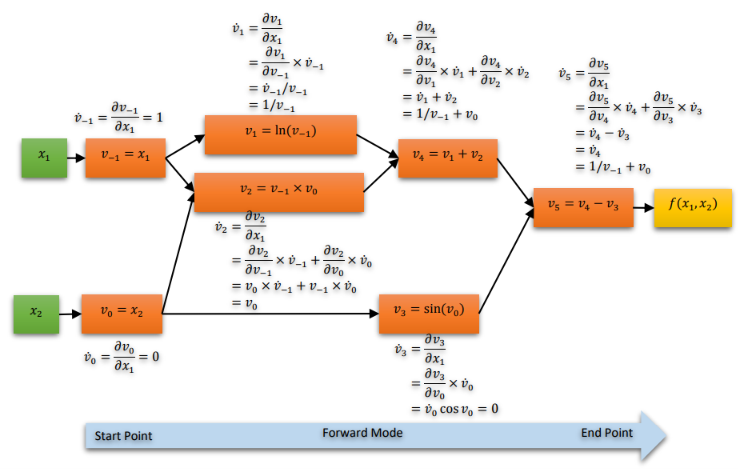
\includegraphics[width=\linewidth]{Images/04_Images/13.png}
    \caption{Ví dụ minh họa chế độ thuận trên đồ thị tính toán của hàm $y = \ln(x_1) + x_1 x_2 - \sin(x_2)$.}
    \label{4.13}
\end{figure}

\paragraph{Tính đạo hàm bằng chế độ đảo\\}

Trong chế độ đảo, quá trình tích lũy đạo hàm được thực hiện theo chiều từ đầu ra về các biến đầu vào. Đặt giá trị liên hợp tại đỉnh $v_i$ là:
\begin{equation}
    \bar{v}_i = \frac{\partial y}{\partial v_i}.
\end{equation}

Trước tiên, giá trị liên hợp tại đỉnh đầu ra được khởi tạo, do $v_5 = y$:
\begin{equation}
    \bar{v}_5 = \frac{\partial y}{\partial v_5} = 1.
\end{equation}

Từ $v_5 = v_4 - v_3$, ta có:
\begin{equation}
    \bar{v}_4 = \bar{v}_5 \frac{\partial v_5}{\partial v_4} = 1(1) = 1,
\end{equation}
và
\begin{equation}
    \bar{v}_3 = \bar{v}_5 \frac{\partial v_5}{\partial v_3} = 1(-1) = -1.
\end{equation}

Tiếp theo, từ $v_4 = v_1 + v_2$:
\begin{equation}
    \bar{v}_1 = \bar{v}_4 \frac{\partial v_4}{\partial v_1} = 1(1) = 1,
\end{equation}
\begin{equation}
    \bar{v}_2 = \bar{v}_4 \frac{\partial v_4}{\partial v_2} = 1(1) = 1.
\end{equation}

Xét nhánh $v_1 = \ln(v_{-1})$:
\begin{equation}
    \bar{v}_{-1}^{(1)} = \bar{v}_1 \frac{\partial v_1}{\partial v_{-1}} = 1\left(\frac{1}{v_{-1}}\right) = \frac{1}{x_1}.
\end{equation}

Xét nhánh $v_2 = v_{-1} v_0$:
\begin{equation}
    \bar{v}_{-1}^{(2)} = \bar{v}_2 \frac{\partial v_2}{\partial v_{-1}} = 1(v_0) = x_2,
\end{equation}
và
\begin{equation}
    \bar{v}_0^{(2)} = \bar{v}_2 \frac{\partial v_2}{\partial v_0} = 1(v_{-1}) = x_1.
\end{equation}

Cuối cùng, xét nhánh $v_3 = \sin(v_0)$:
\begin{equation}
    \bar{v}_0^{(3)} = \bar{v}_3 \frac{\partial v_3}{\partial v_0} = -1(\cos(v_0)) = -\cos(x_2).
\end{equation}

Do $v_{-1} = x_1$ và $v_0 = x_2$, các đóng góp tại mỗi biến đầu vào được cộng dồn lại. Đối với $x_1$:
\begin{equation}
\begin{aligned}
    \frac{\partial y}{\partial x_1} &= \bar{v}_{-1} = \bar{v}_{-1}^{(1)} + \bar{v}_{-1}^{(2)} \\
    &= \frac{1}{x_1} + x_2.
\end{aligned}
\end{equation}

Đối với $x_2$:
\begin{equation}
\begin{aligned}
    \frac{\partial y}{\partial x_2} &= \bar{v}_0 = \bar{v}_0^{(2)} + \bar{v}_0^{(3)} \\
    &= x_1 - \cos(x_2).
\end{aligned}
\end{equation}

Do đó, chế độ đảo cũng thu được kết quả đồng nhất:
\begin{equation}
    \nabla f(x_1,x_2) = 
    \begin{bmatrix}
        \dfrac{1}{x_1} + x_2 \\[6pt]
        x_1 - \cos(x_2)
    \end{bmatrix}.
    \label{eq:reverse_gradient}
\end{equation}

Chi tiết quá trình tính toán các giá trị và tích lũy các giá trị các biến liên hợp theo chiều đảo tại điểm $(x_1,x_2) = (2,5)$ nhằm xác định các đạo hàm riêng của hàm đầu ra $y$ đối với các biến đầu vào $x_1$ và $x_2$.

\begin{table}[H]
\centering
\renewcommand{\arraystretch}{1.35} 
\begin{tabular*}{\textwidth}{@{\extracolsep{\fill}} l l | l l @{}}
\hline
\multicolumn{2}{l|}{Chuỗi giá trị các biến tính toán} & \multicolumn{2}{l}{Chuỗi giá trị các biến trung gian} \\
\hline
$v_{-1} = x_1$        & $= 2$             & $\bar{v}_5 = \bar{y}$                                                               & $= 1$ \\
$v_0 = x_2$           & $= 5$             & $\bar{v}_4 = \bar{v}_5 \frac{\partial v_5}{\partial v_4}$                           & $= 1 \times 1 = 1$ \\
$v_1 = \ln(v_{-1})$   & $\approx 0.693$   & $\bar{v}_3 = \bar{v}_5 \frac{\partial v_5}{\partial v_3}$                           & $= 1 \times (-1) = -1$ \\
$v_2 = v_{-1} \times v_0$& $= 10$         & $\bar{v}_2 = \bar{v}_4 \frac{\partial v_4}{\partial v_2}$                           & $= 1 \times 1 = 1$ \\
$v_3 = \sin(v_0)$     & $\approx -0.959$  & $\bar{v}_1 = \bar{v}_4 \frac{\partial v_4}{\partial v_1}$                           & $= 1 \times 1 = 1$ \\
$v_4 = v_1 + v_2$     & $\approx 10.693$  & $\bar{v}_0 = \bar{v}_2 \frac{\partial v_2}{\partial v_0} + \bar{v}_3 \frac{\partial v_3}{\partial v_0}$ & $= 1(2) + (-1)\cos(5) \approx 1.716$ \\
$v_5 = v_4 - v_3$     & $\approx 11.652$  & $\bar{v}_{-1} = \bar{v}_1 \frac{\partial v_1}{\partial v_{-1}} + \bar{v}_2 \frac{\partial v_2}{\partial v_{-1}}$ & $= 1(0.5) + 1(5) = 5.5$ \\
$y = v_5$             & $\approx 11.652$  & $\bar{\mathbf{x}} = (\bar{v}_{-1}, \bar{v}_0)$                                      & $= (5.5, \; 1.716)$ \\
\hline
\end{tabular*}
\caption{Ví dụ minh họa vi phân tự động ở chế độ đảo đối với hàm $y = f(x_1,x_2) = \ln(x_1) + x_1 x_2 - \sin(x_2)$ tại điểm $(x_1,x_2) = (2,5)$.}
\end{table}

\begin{figure}[H]
    \centering
    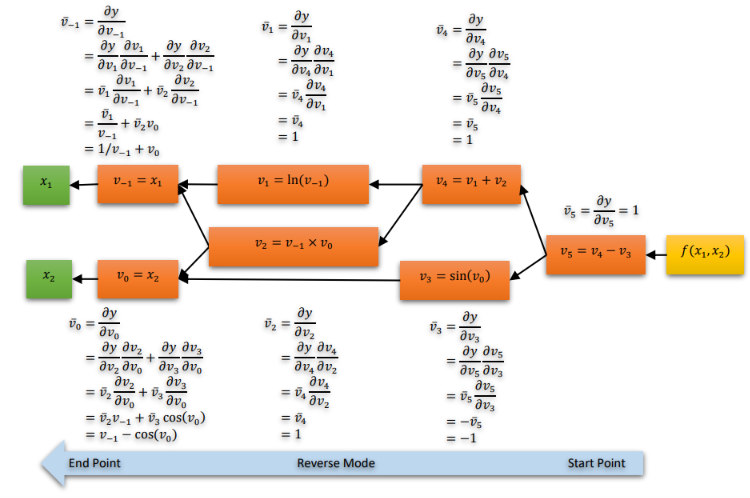
\includegraphics[width=\linewidth]{Images/04_Images/14.png}
    \caption{Ví dụ về chế độ đảo vi phân tự động trên đồ thị tính toán của hàm $y = \ln(x_1) + x_1 x_2 - \sin(x_2)$.}
    \label{4.14}
\end{figure}

\begin{lstlisting}[caption=Cài đặt chế độ thuận bằng thư viện NumPy]
import numpy as np

# --- (x_1,x_2) = (2,5) ---
x1, x2 = 2.0, 5.0

# --- Forward ---
# --- y = f(x_1,x_2) = ln(x_1) + x_1 x_2 - sin(x_2) ---
v1 = np.log(x1)
v2 = x1 * x2
v3 = np.sin(x2)
v4 = v1 + v2
y  = v4 - v3

# --- Forward mode x1 ---
dv1 = 1 / x1
dv2 = x2
dv3 = 0
dv4 = dv1 + dv2
dy_dx1 = dv4 - dv3

# --- Forward mode x2 ---
dv1 = 0
dv2 = x1
dv3 = np.cos(x2)
dv4 = dv1 + dv2
dy_dx2 = dv4 - dv3

# --- In cac gia tri ---
print(y)
print(dy_dx1, dy_dx2)
\end{lstlisting}

\begin{lstlisting}[caption=Cài đặt chế độ đảo bằng thư viện NumPy]
import numpy as np

# --- (x_1,x_2) = (2,5) ---
x1, x2 = 2.0, 5.0


# --- Reverse pass ---
# --- y = f(x_1,x_2) = ln(x_1) + x_1 x_2 - sin(x_2) ---
bar_v5 = 1.0

bar_v4 = bar_v5
bar_v3 = -bar_v5

bar_v1 = bar_v4
bar_v2 = bar_v4

bar_v_minus1 = bar_v1 * (1 / x1) + bar_v2 * x2
bar_v0 = bar_v2 * x1 + bar_v3 * np.cos(x2)

# --- In cac gia tri ---
print(bar_v_minus1, bar_v0)
\end{lstlisting}

\begin{lstlisting}[caption= Cơ chế vi phân tự động bằng PyTorch]
import torch

# --- (x_1,x_2) = (2,5) ---
x = torch.tensor([2.0, 5.0], requires_grad=True)

# --- y = f(x_1,x_2) = ln(x_1) + x_1 x_2 - sin(x_2) ---
y = torch.log(x[0]) + x[0] * x[1] - torch.sin(x[1])

y.backward()

# --- In cac gia tri ---
print(y.item())
print(x.grad)
\end{lstlisting}